\documentclass[11pt]{book}

% Use the ETAMU physics style package
\usepackage{../../shared/styles/etamu-physics}
\usepackage{lscape}
\usepackage{tikz}
\usepackage{pgfplots}

% Document metadata
\title{University Physics I\\Instructor Manual}
\author{ETAMU Department of Physics and Astronomy}
\date{\today}

\begin{document}

\frontmatter
\maketitle

\begin{landscape}
\begin{center}
\begin{tikzpicture}[scale=5, every node/.style={font=\Huge}]
    % Triangle sides
    \draw[thick] (0,0) -- (3,0) -- (3,2) -- cycle;
    % Hypotenuse vector
    \draw[->, >=Stealth, very thick, blue] (0,0) -- (3,2) node[midway, above left] {$\vec{A}$};
    % Base
    \draw[->, >=Stealth, very thick] (0,0) -- (3,0);
    % Height
    \draw[->, >=Stealth, very thick] (3,0) -- (3,2);
    % Angle theta at origin
    \draw (0.4,0) arc (0:33.69:0.4);
    \node at (0.55,0.18) {$\theta$};
    % Angle phi at top right
    \draw (3,1.5) arc (-90:-158:0.4);
    \node at (2.75,1.45) {$\phi$};
    % Dotted lines for clarity
    \draw[dashed] (0,0) -- (3,2);
    % Labels for triangle sides
    \node at (1.5, -0.18) {$A_x = A \cos\theta$};
    \node at (1.625, -0.38) {$ = A \sin\phi$};
    \node[rotate=-90] at (3.18,1) {$A_y = A \sin\theta$};
    \node[rotate=-90] at (3.38,0.85) {$= A \cos\phi$};
    % Title below
    \node at (1.5, -0.75) {\Large Right Triangle with Angles $\theta$ and $\phi$};
\end{tikzpicture}
\end{center}
\end{landscape}

\tableofcontents

\chapter{Preface}

This is the instructor manual for ETAMU's University Physics I (PHYS 2425) studio-mode course.
This manual is intended to be used as a guide for instructors teaching the course, as well as 
undergraduate learning assistants (LAs) and graduate teaching assistants (TAs) who may be helping
to facilitate the course. \\

In this manual, you will find brief descriptions of each assignment students will complete in class,
as well as additional details about each assignment that may be helpful for instructors.  This includes
tips for facilitating group work, common student misconceptions, and additional resources for instructors. \\

This manual is not intended to be used as a solution manual.  First, if this manual were to be released to students,
we would need to re-write all the problems to ensure students are not simply copying answers. Second, the best way 
to really understand the problems is to work through them yourself.  This will help you better facilitate group work
and guide students to the correct answers.  In a few cases, a specific solution is provided to illustrate an important
point, but in general, you should work through the problems yourself. \\

If you have any questions or feedback about this manual, please feel free to reach out to the ETAMU Physics Department. 
This manual is written in LaTeX, and the source files are available on GitHub, link below. \\

https://github.com/Blake-Head/ETAMU-Physics.git \\

While it goes without saying, please do not share this manual or any of its contents with students.  Doing so
would seriously undermine the integrity of the course.  If you are an instructor, TA, or LA for the course, please keep this manual
private. \\



\newpage
\section{Ordering of Topics}

The ordering of topics in this course is not set in stone.  The following is a suggested order
that has been found to work well.  However, you may find that a different order works better
for you and your students.  Feel free to adjust the order as needed. \\ 

\begin{enumerate}
    \item \textbf{Momentum and Impulse} (About 3 Weeks)
        \begin{itemize}
            \item Momentum and Impulse
            \item Momentum Conservation
            \item Vectors
        \end{itemize}
    \item \textbf{Dynamics} (About 4 Weeks)
        \begin{itemize}
            \item Newton's Laws
            \item Free Body Diagrams
            \item Friction 
            \item Uniform Circular Motion
        \end{itemize}
    \item \textbf{Work and Energy} (About 3 Weeks)
        \begin{itemize}
            \item Work Energy Theorem
            \item Work from Constant and Varying Forces
            \item Conservation of Energy
        \end{itemize}
    \item \textbf{Kinematics} (About 4 Weeks)
        \begin{itemize}
            \item Displacement, Velocity, Acceleration
            \item Motion with Constant Acceleration
            \item Problem Solving with Kinematics
        \end{itemize}
    \item \textbf{Rotational Motion} (About 2 Weeks)
        \begin{itemize}
            \item Torque
            \item Angular Momentum and Moment of Inertia
            \item Rotational Kinematics
        \end{itemize}
\end{enumerate}

If you are from the future, you may note the lack of sections on thermodynamics, fluids, and waves.  These sections
have been intentionally left out of this course, as they are typically covered in other courses.  If you have time to 
include more material, thermodynamics is a good choice.

\newpage
\section*{A Note on Ordering}
This ordering is chosen as, at the time of writing, University Physics 1 requires Calculus 1
as a co-requisite.  This means that students will be learning about derivatives and integrals
for the first time while taking this course.  The ordering above allows students to learn
about momentum and impulse first, which can be done with only algebra.  This allows students
to get comfortable with the studio format and group work before being introduced to more
mathematically complex topics. \\

That being said, one could easily introduce the concept of simple derivatives and integrals
up front.  The most complex calculus needed is the ability to integrate / differentiate polynomials. 
There are a few example problems that ask for exponentials and trigonometric functions, but these are 
primarily for practice and can be easily skipped. \\

Given the structure of all the course materials, none assume prior knowledge of the previous section(s),
which as a physicist you likely know is because most of this is just momentum conservation in disguise.
Each module can, for the most part, be taught independently of the others. Of course, use your own judgment and adapt as needed.






\mainmatter

% Include chapters from separate files

\input{chapters/momentum.tex}
\chapter{Dynamics}
This is the first experiment chapter. Add your content here.

\section{Energy and Work}

The work-energy theorem states that the work done on an object equals its change in kinetic energy:

\[ W = \Delta KE = \frac{1}{2}mv_f^2 - \frac{1}{2}mv_i^2 \]

\begin{tutorialbox}[title=Creating Energy Diagrams]
Use PGFPlots for energy graphs:
\begin{verbatim}
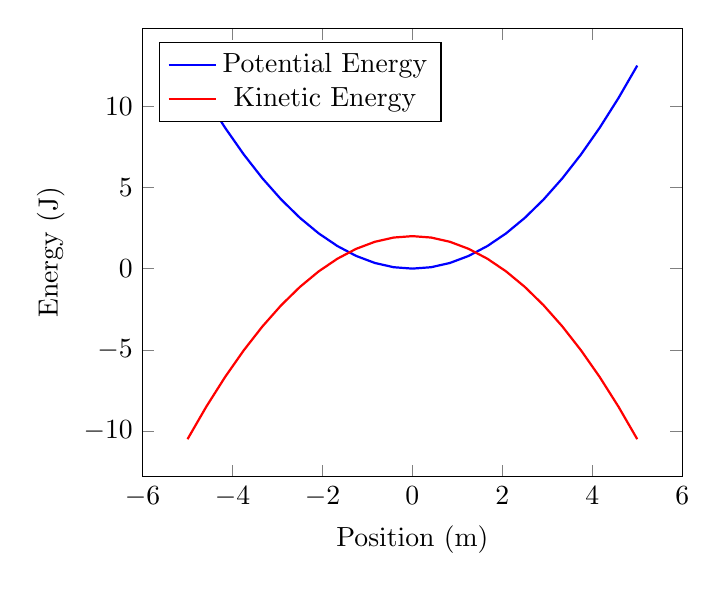
\begin{tikzpicture}
\begin{axis}[
    xlabel={Position (m)},
    ylabel={Energy (J)},
    legend pos=north west
]
\addplot[blue,thick] {x^2/2};
\addlegendentry{Potential Energy}
\addplot[red,thick] {2-x^2/2};
\addlegendentry{Kinetic Energy}
\end{axis}
\end{tikzpicture}
\end{verbatim}
\end{tutorialbox}

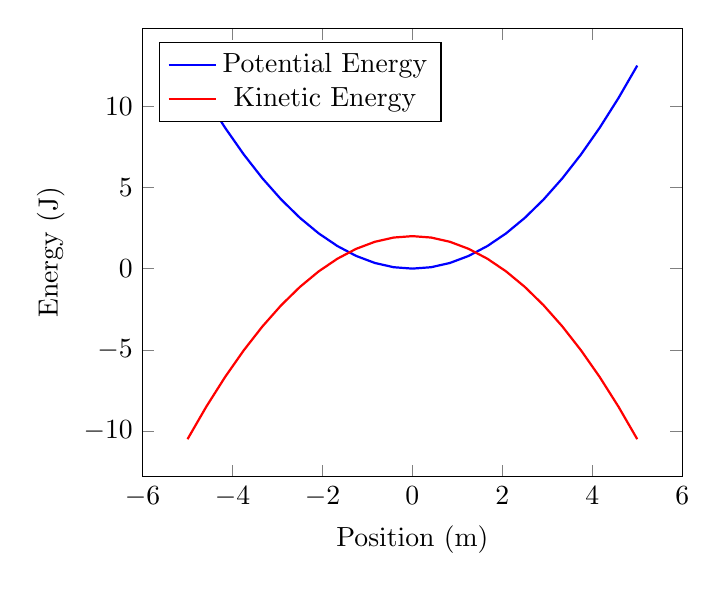
\begin{tikzpicture}
\begin{axis}[
    xlabel={Position (m)},
    ylabel={Energy (J)},
    legend pos=north west
]
\addplot[blue,thick] {x^2/2};
\addlegendentry{Potential Energy}
\addplot[red,thick] {2-x^2/2};
\addlegendentry{Kinetic Energy}
\end{axis}
\end{tikzpicture}
\chapter{Work and Energy}
Content to be added here.
\chapter{Kinematics}
content to be added here.
\chapter{Rotational Motion}
Content to be added here.


\backmatter

\appendix


\end{document}